In this section, the goal is to explore in details the SRI configurations which are available for testing purposes. Tests will be done on both CPU-miner and real ASIC machine (Antminer S19J Pro), following the official \textit{Getting Started} guide which can be found at \cite{stratumprotocolStratumV2}.

\subsection{Testing SRI configurations}
SRI working group currently developed and shipped all the roles which are needed for every of the 4 configurations introduced in the previous section. However, the ones which will be tested here, are the \textbf{Config C and D}, since they are the most ready and documented for testing on real ASIC machines.\\
To start testing also Config A and B, of course, it's possible to run every individual role, following the indications reported in the README of them (e.g. for the SV2 Mining Proxy, follow the guidelines on the official SRI Github repository).\\

\subsubsection{Prerequisites}
Before entering the Configurations details, there are some first-steps that needs to be checked:
\begin{itemize}
    \item Rust installed: if not, install it by running this command in the terminal:
    \begin{lstlisting}[style=bashStyle, numbers=none]
        curl --proto '=https' --tlsv1.2 -sSf https://sh.rustup.rs | sh
    \end{lstlisting}
    \item Clone the SRI repository locally:
    \begin{lstlisting}[style=bashStyle, numbers=none]
        git clone https://github.com/stratum-mining/stratum.git 
    \end{lstlisting}
\end{itemize}
At this point everything is correctly setup and ready for the testing phase.\\

\subsubsection{Config C}
This configuration, as seen in \ref{configC}, allows Mining Devices running SV1 firmware to connect to a SV2 Pool through a Translation Proxy (tProxy). The proxy is designed to sit in between a SV1 downstream role (most typically Mining Device(s) running SV1 firmware) and a SV2 upstream role (most typically a SV2 Pool Server).\\
In this case, since there is not intended to be a Template Provider miner-side, transactions selections is delegated to the SV2 Pool server, which is running its local Template Provider, as explained in Figure \ref{fig:SRI_configC}.\\\\
First of all, once the SRI project repository just cloned is accessed, the \textbf{SV2 Pool server has to be run}:
\begin{lstlisting}[style=bashStyle, numbers=none]
    cd stratum/roles/v2/pool/
    cp pool-config-example.toml ./conf/pool-config.toml
    cd conf/
\end{lstlisting}
Now the example config file called \textit{pool-config.toml} is copied into the \textit{/conf} directory. This file contains all the parameters needed for the pool to be correctly configured. It's possible to enter the file and customize it for the most desired behaviour, following the guidelines available in the README file of the pool role.
For simplicity, it's possible to use the \textbf{testnet} Template Provider which is hosted by the SRI working group: in this way it's not needed to be run a local one. To do that, it's needed to comment the line corresponding to \textit{tp\_address = "127.0.0.1:8442"}, and uncomment the one which corresponds to \textit{tp\_address = "89.116.25.191:8442"}. \\\\
After that, to finally run the SV2 Pool:
\begin{lstlisting}[style=bashStyle, numbers=none]
    cargo run -p pool_sv2 
\end{lstlisting}
As described in the command output, the Pool is now connected to the hosted testnet Template Provider, and it will get the transactions to be put in the next block template from it.\\ Now the Pool is ready to get connection requests, listening on the port 342254.    
\begin{figure}[h!]
    \centering
    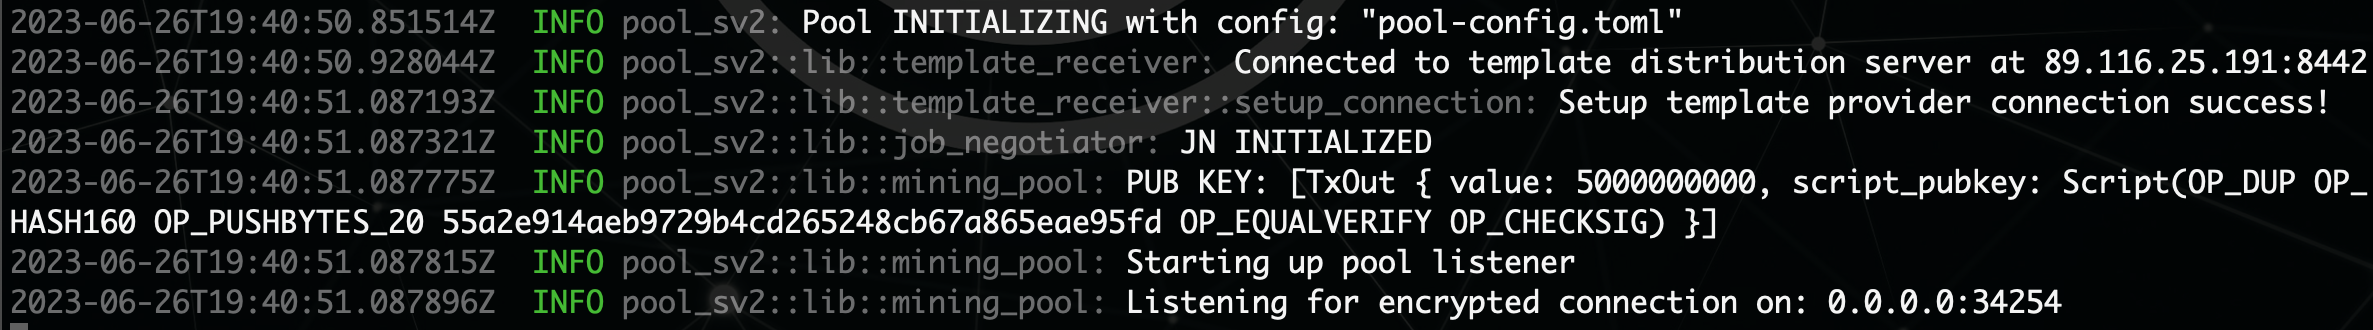
\includegraphics[width=15cm]{Figures/sri/configC_1.png}
    \caption{SV2 Pool connected to the hosted Template Provider, \textit{config C}}
    \label{fig:configC_1}
\end{figure}
\newline
\noindent At this point, since will be used SV1 Mining Devices, \textbf{the Translator Proxy is needed}. In a new terminal:
\begin{lstlisting}[style=bashStyle, numbers=none]
    cd stratum/roles/translator/
    cp proxy-config-example.toml ./conf/proxy-config.toml
    cd conf/
\end{lstlisting}
Since the configuration file provided is already prepared for the Config C, the Translator Proxy is ready to be run:
\begin{lstlisting}[style=bashStyle, numbers=none]
    cargo run -p translator_sv2 
\end{lstlisting}
The Translator Proxy is now running, and as can be seen in the command output, it has requested a connection to the SV2 Pool, asking to open an \textit{extended channel} \cite{githubSv2spec05MiningProtocolmdMain}, and it received an \textit{extended mining job}, and a \textit{prev hash}. So it's now ready to customize the templates that it will distribute to the Mining Devices which will be connected to it!\\   

\textbf{Note}: to learn more about the messages exchanged during this phase, look at:
\begin{itemize}
    \item \textit{Setup connection} message
    \item \textit{OpenExtendedMiningChannel} message
    \item \textit{NewMiningJob} message 
    \item \textit{SetNewPrevHash} message\\\\
    All the messages details are well explained in the SV2 mining protocol specifications repository.
\end{itemize}
\begin{figure}[h!]
    \centering
    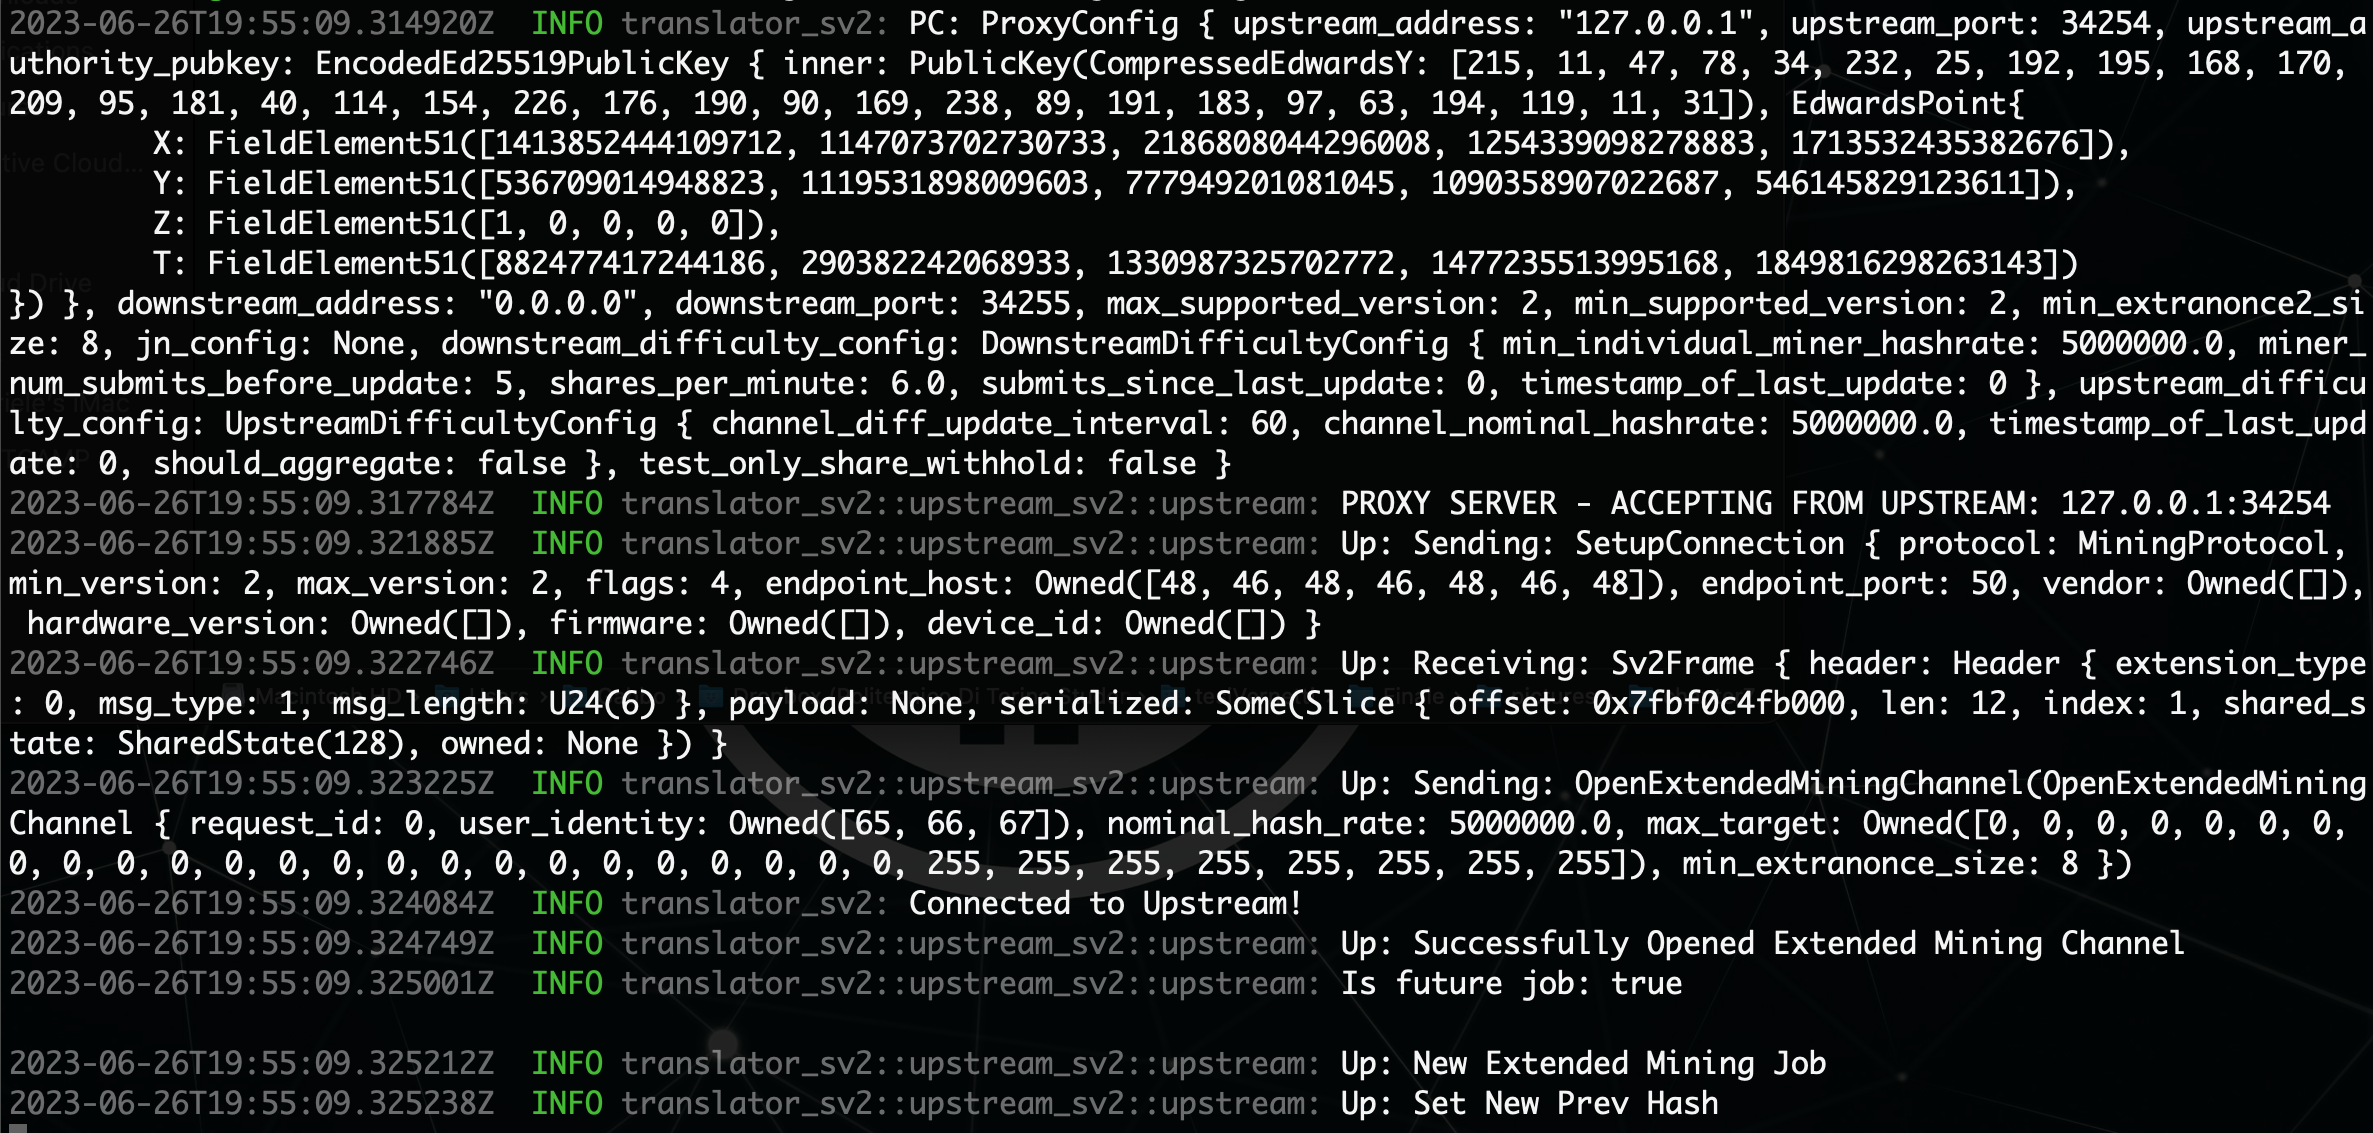
\includegraphics[width=15cm]{Figures/sri/configC_2.png}
    \caption{Translator Proxy connected to the SV2 Pool, \textit{config C}}
    \label{fig:configC_2}
\end{figure}

\noindent Now, the only role which is missing is the \textbf{SV1 Mining Device}. There are two alternatives to run it:
\begin{itemize}
    \item \textbf{CPU-miner}\\
    An open-source SHA-256, multi-threaded CPU-miner for Bitcoin which works following the Stratum (V1) protocol. Once downloaded, in a new terminal:
    \begin{lstlisting}[style=bashStyle, numbers=none]
    cd Downloads/
    ./minerd -a sha256d -o stratum+tcp://localhost:34255 -q -D -P
    \end{lstlisting}
    \begin{figure}[h!]
    \centering
    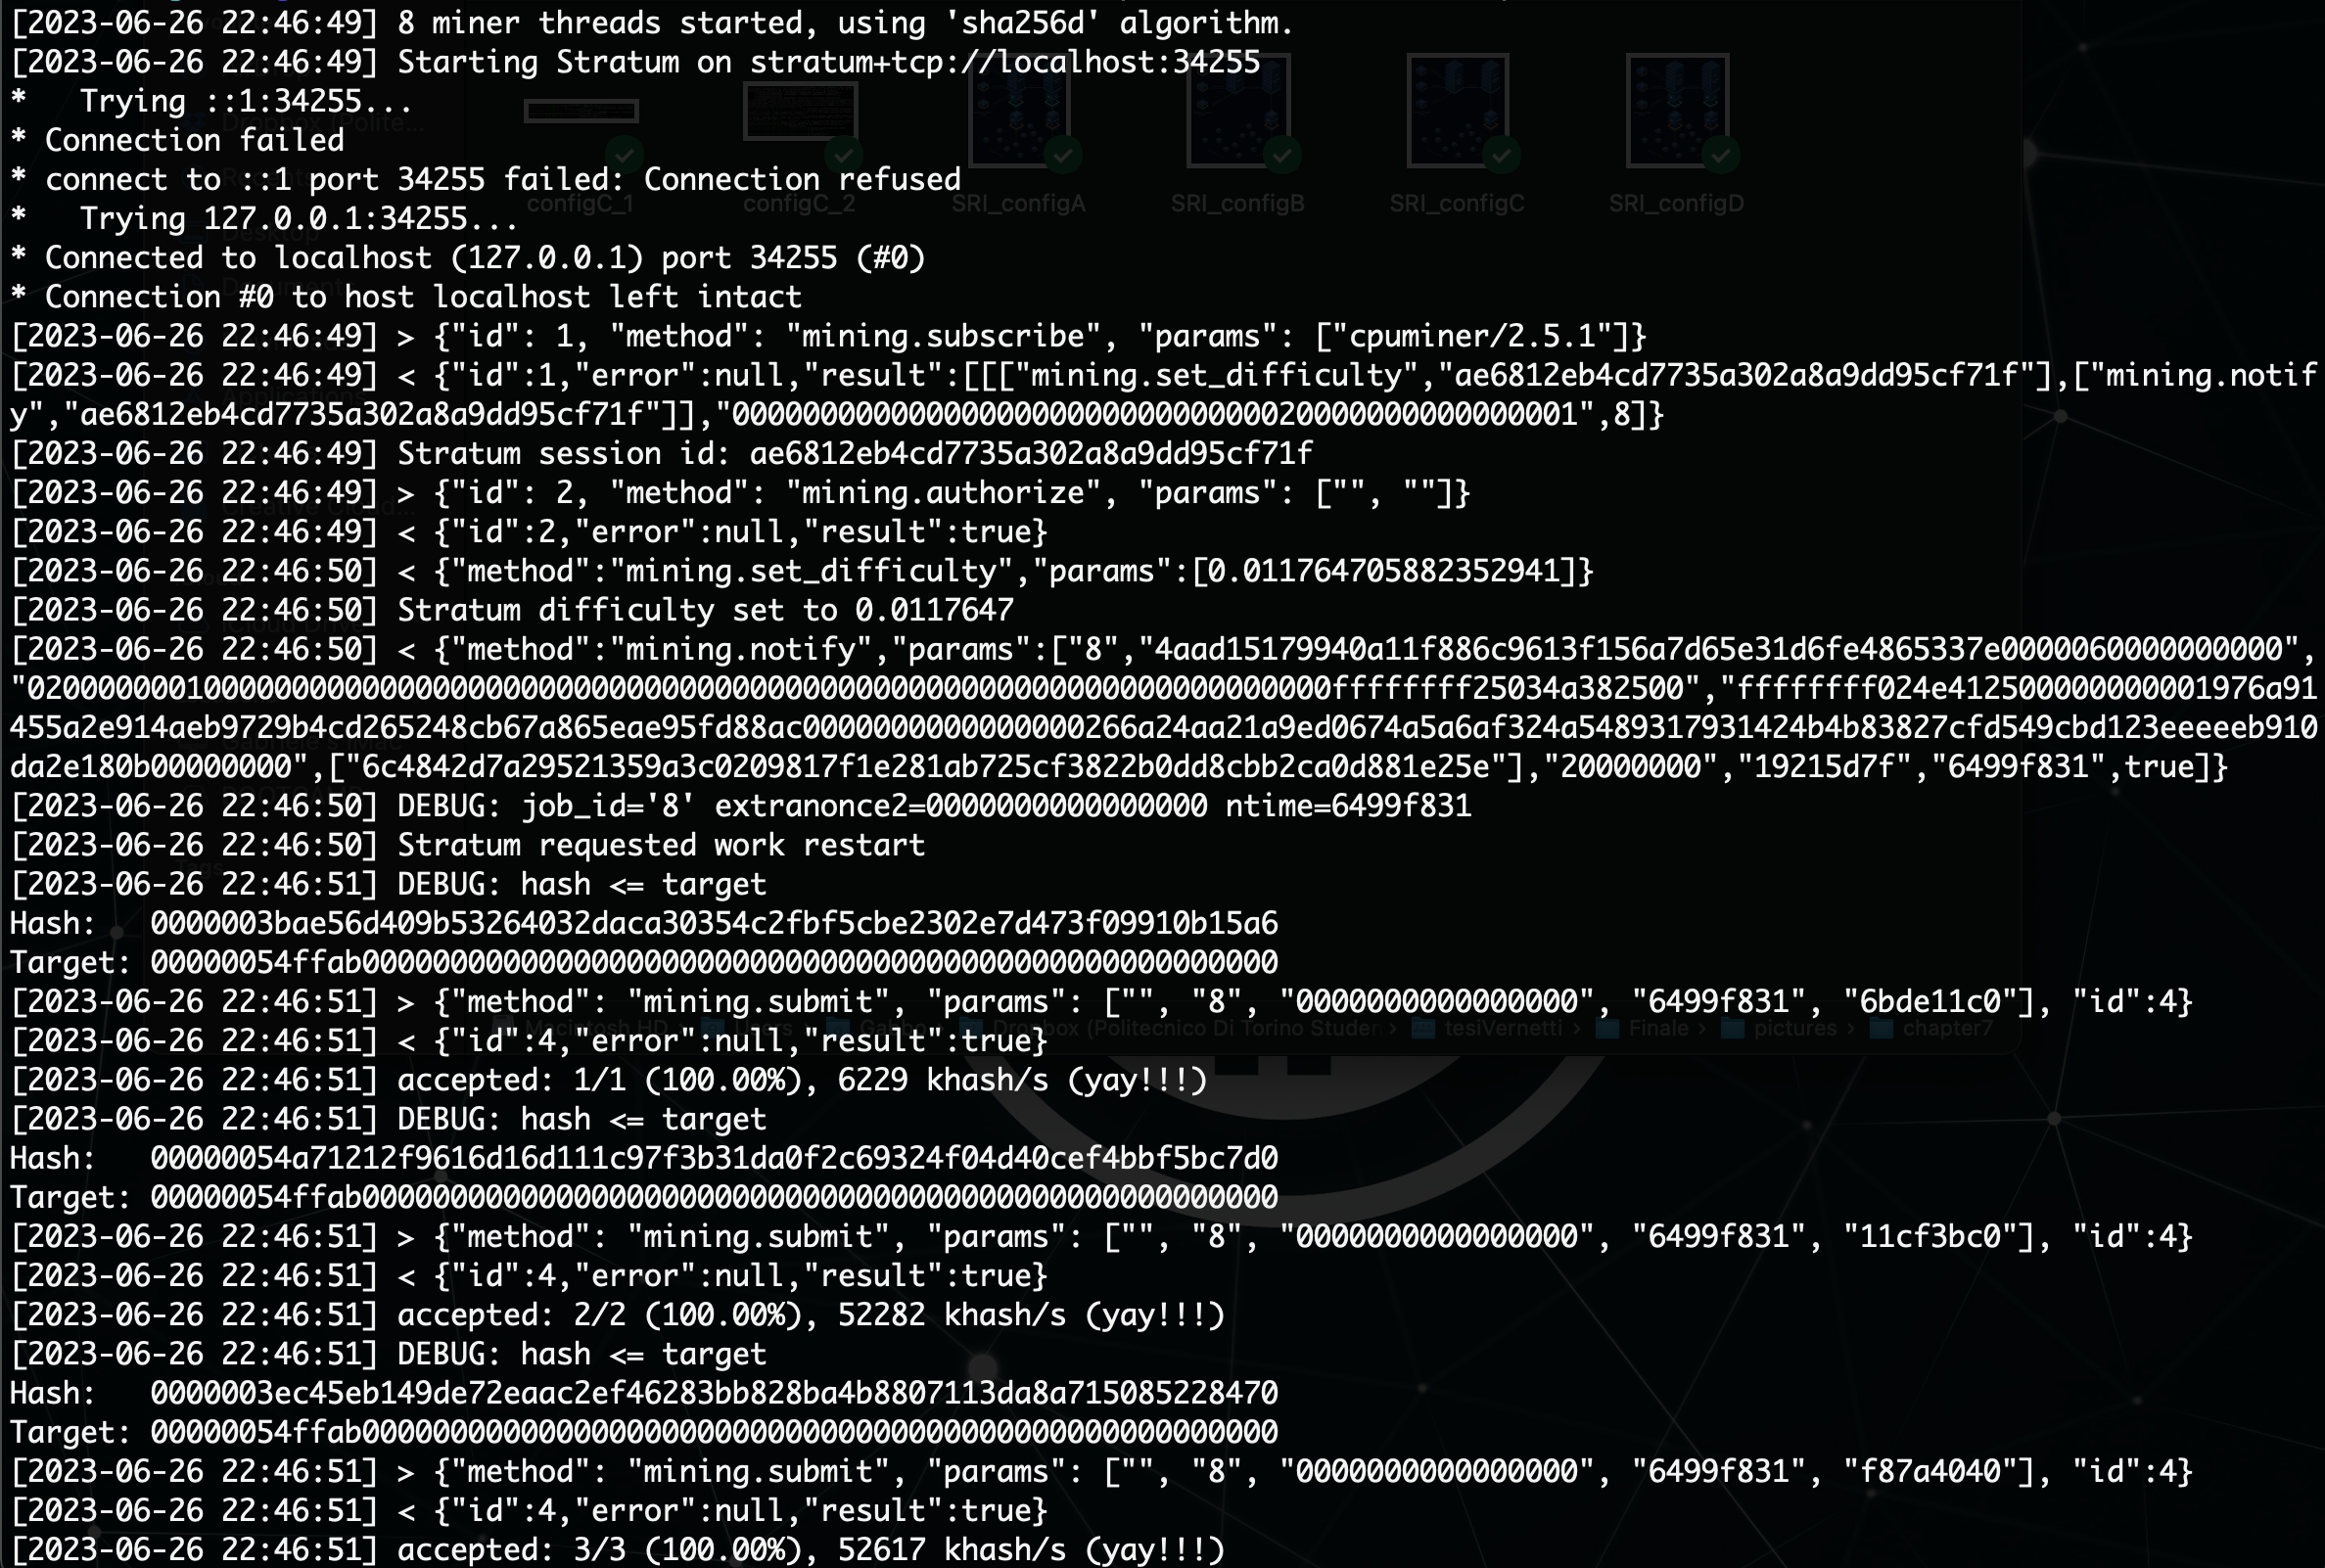
\includegraphics[width=15cm]{Figures/sri/configC_3.png}
    \caption{SV1 CPU-miner running, using the Translation Proxy, \textit{config C}}
    \label{fig:cpuminer}
    \end{figure}
    As described in the Figure \ref{fig:cpuminer}, the SV1 CPU-miner is running correctly: it connected to the Translator Proxy on port 34255, doing the subscription and receiving a new job with the \textit{mining.notify} SV1 message.
    Then, it started working and sending shares to the tProxy, with the \textit{mining.submit} SV1 message.

    
    \item \textbf{ASIC miner}\\
    With a real ASIC machine, it's very easy to configure it to point to the Translator Proxy. In the miner pool settings, the following string has to be added to the current endpoints:
    \begin{lstlisting}[style=bashStyle, numbers=none]
    stratum+tcp://<tProxy ip>:34255
    \end{lstlisting}

    \begin{figure}[h!]
    \centering
    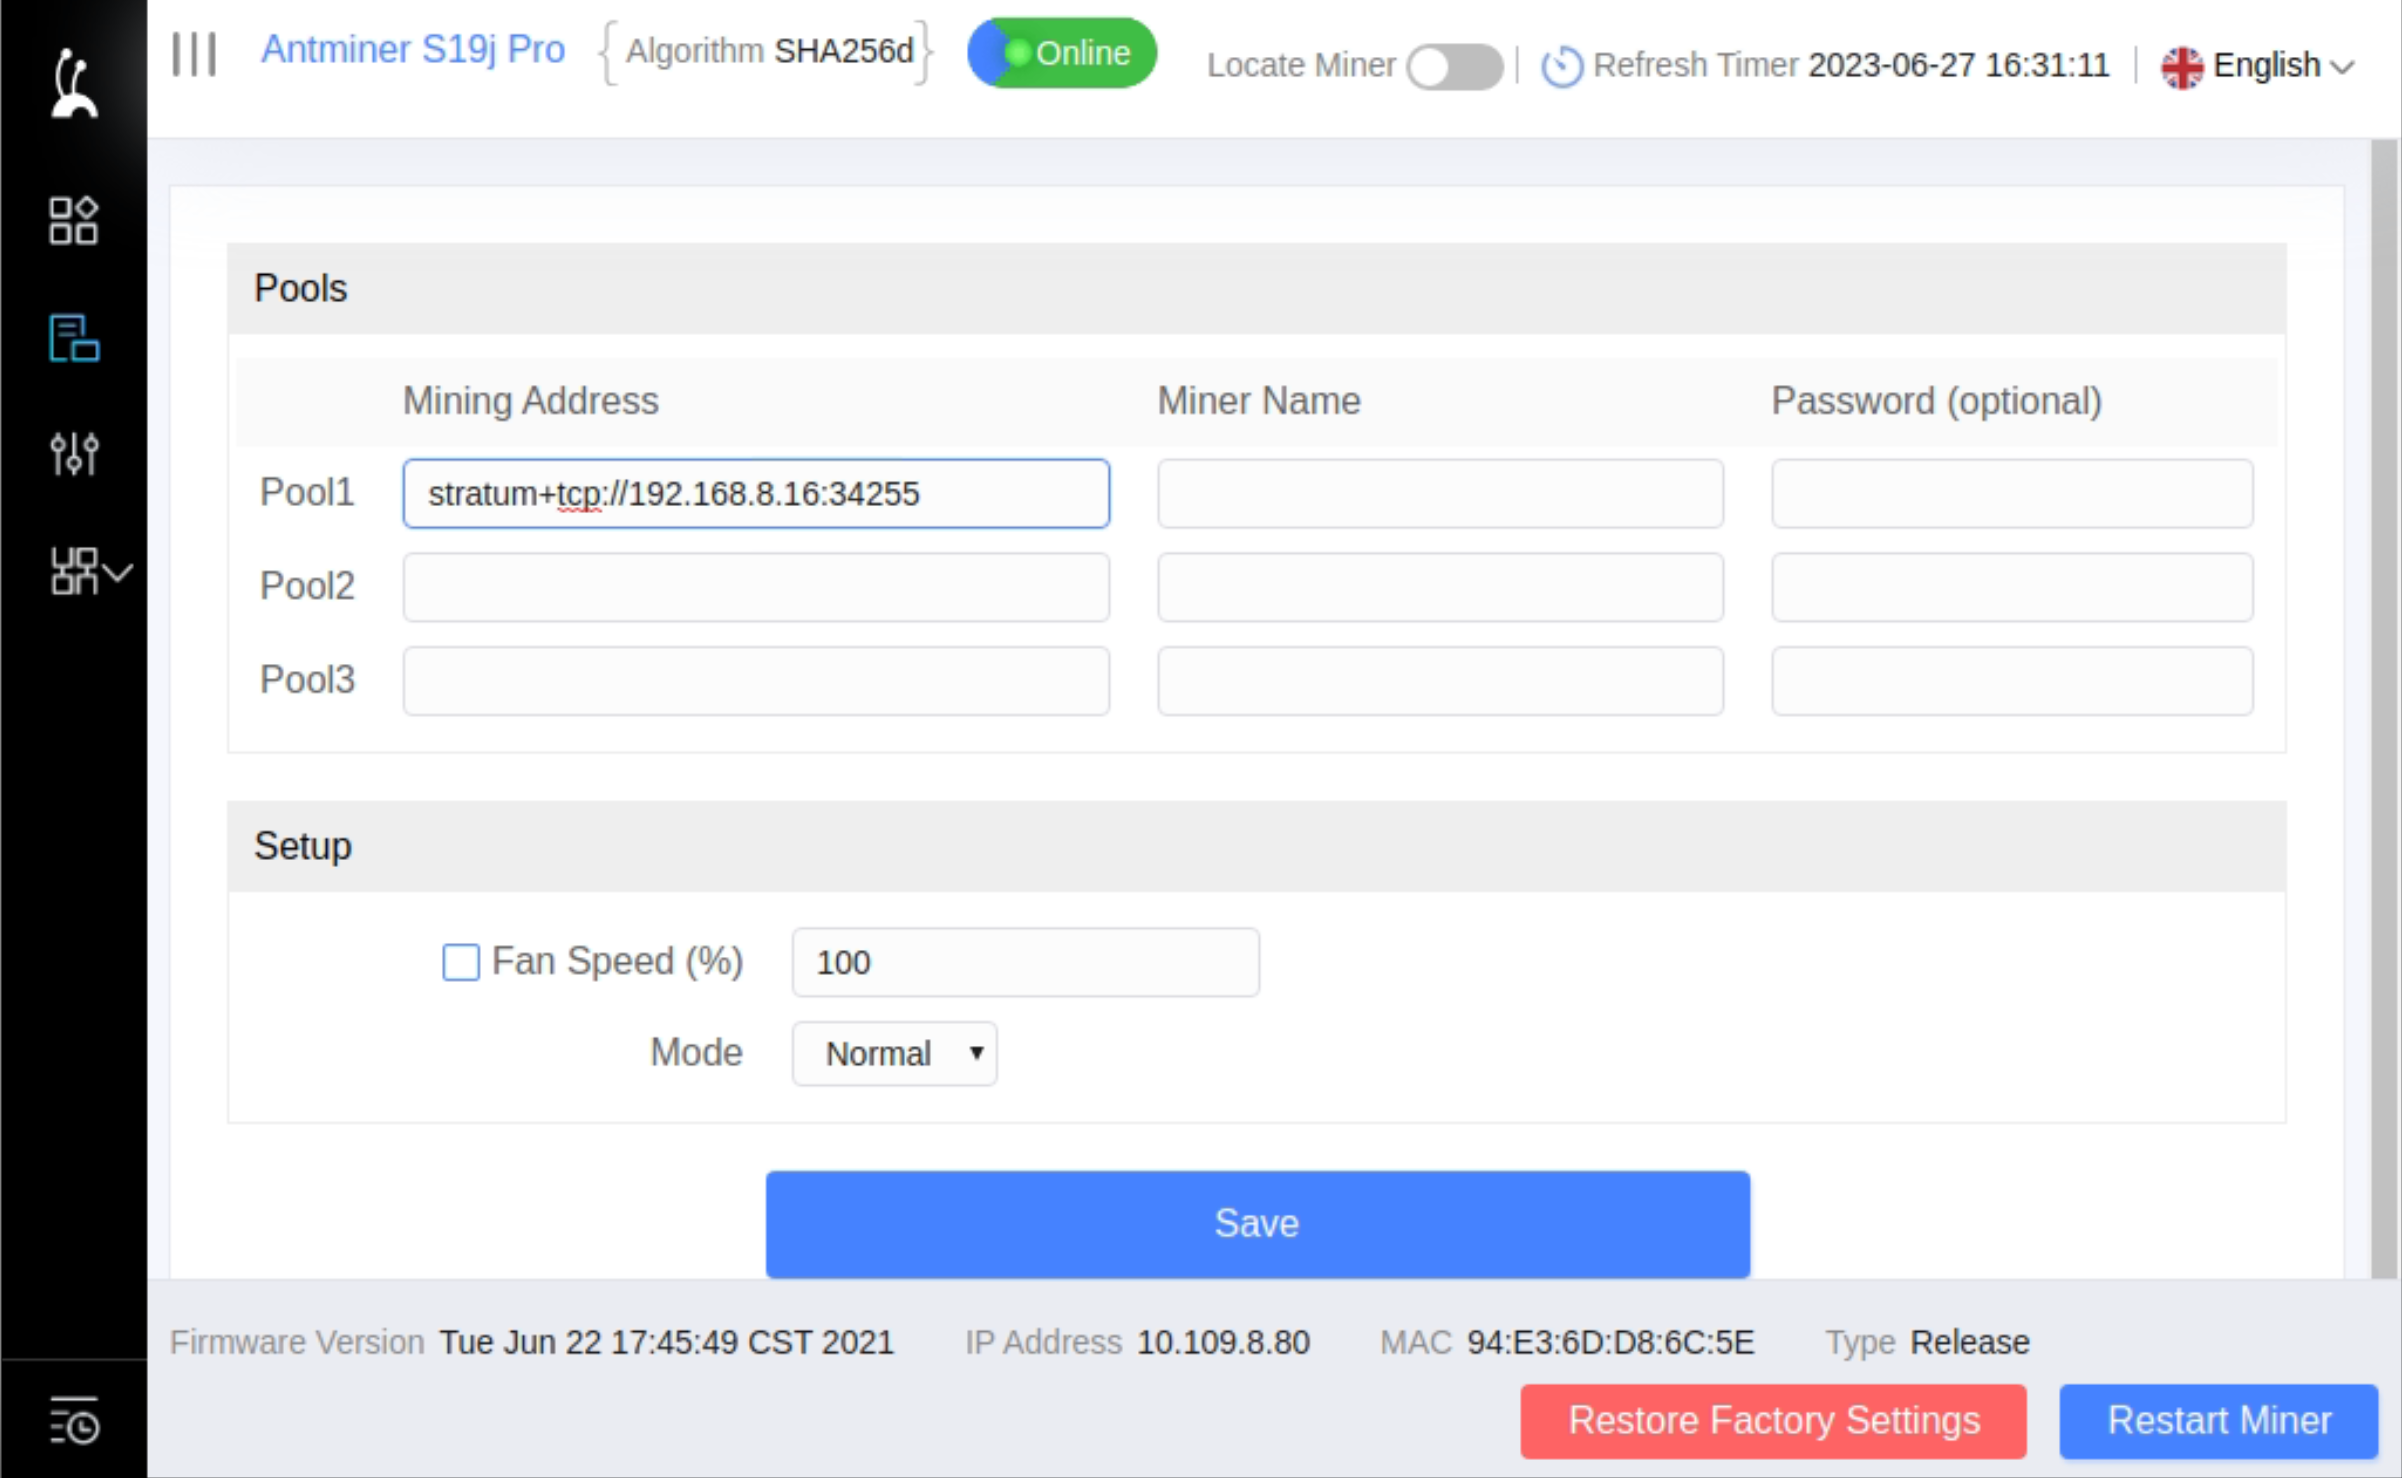
\includegraphics[width=15cm]{Figures/sri/sri_miner.png}
    \caption{Pool settings of a Antminer S19J Pro}
    \label{fig:antminer}
    \end{figure}

    Once configured, the ASIC miner will restart automatically and it will point its hashrate to the Translator Proxy IP previously set.\\
    As captioned in Figure \ref{fig:sri_asic_proxy}, the Translator Proxy logs correctly the connection request coming from the machine, parsing the SV1 messages (subscribe, authorize, etc.).
    \begin{figure}[h!]
    \centering
    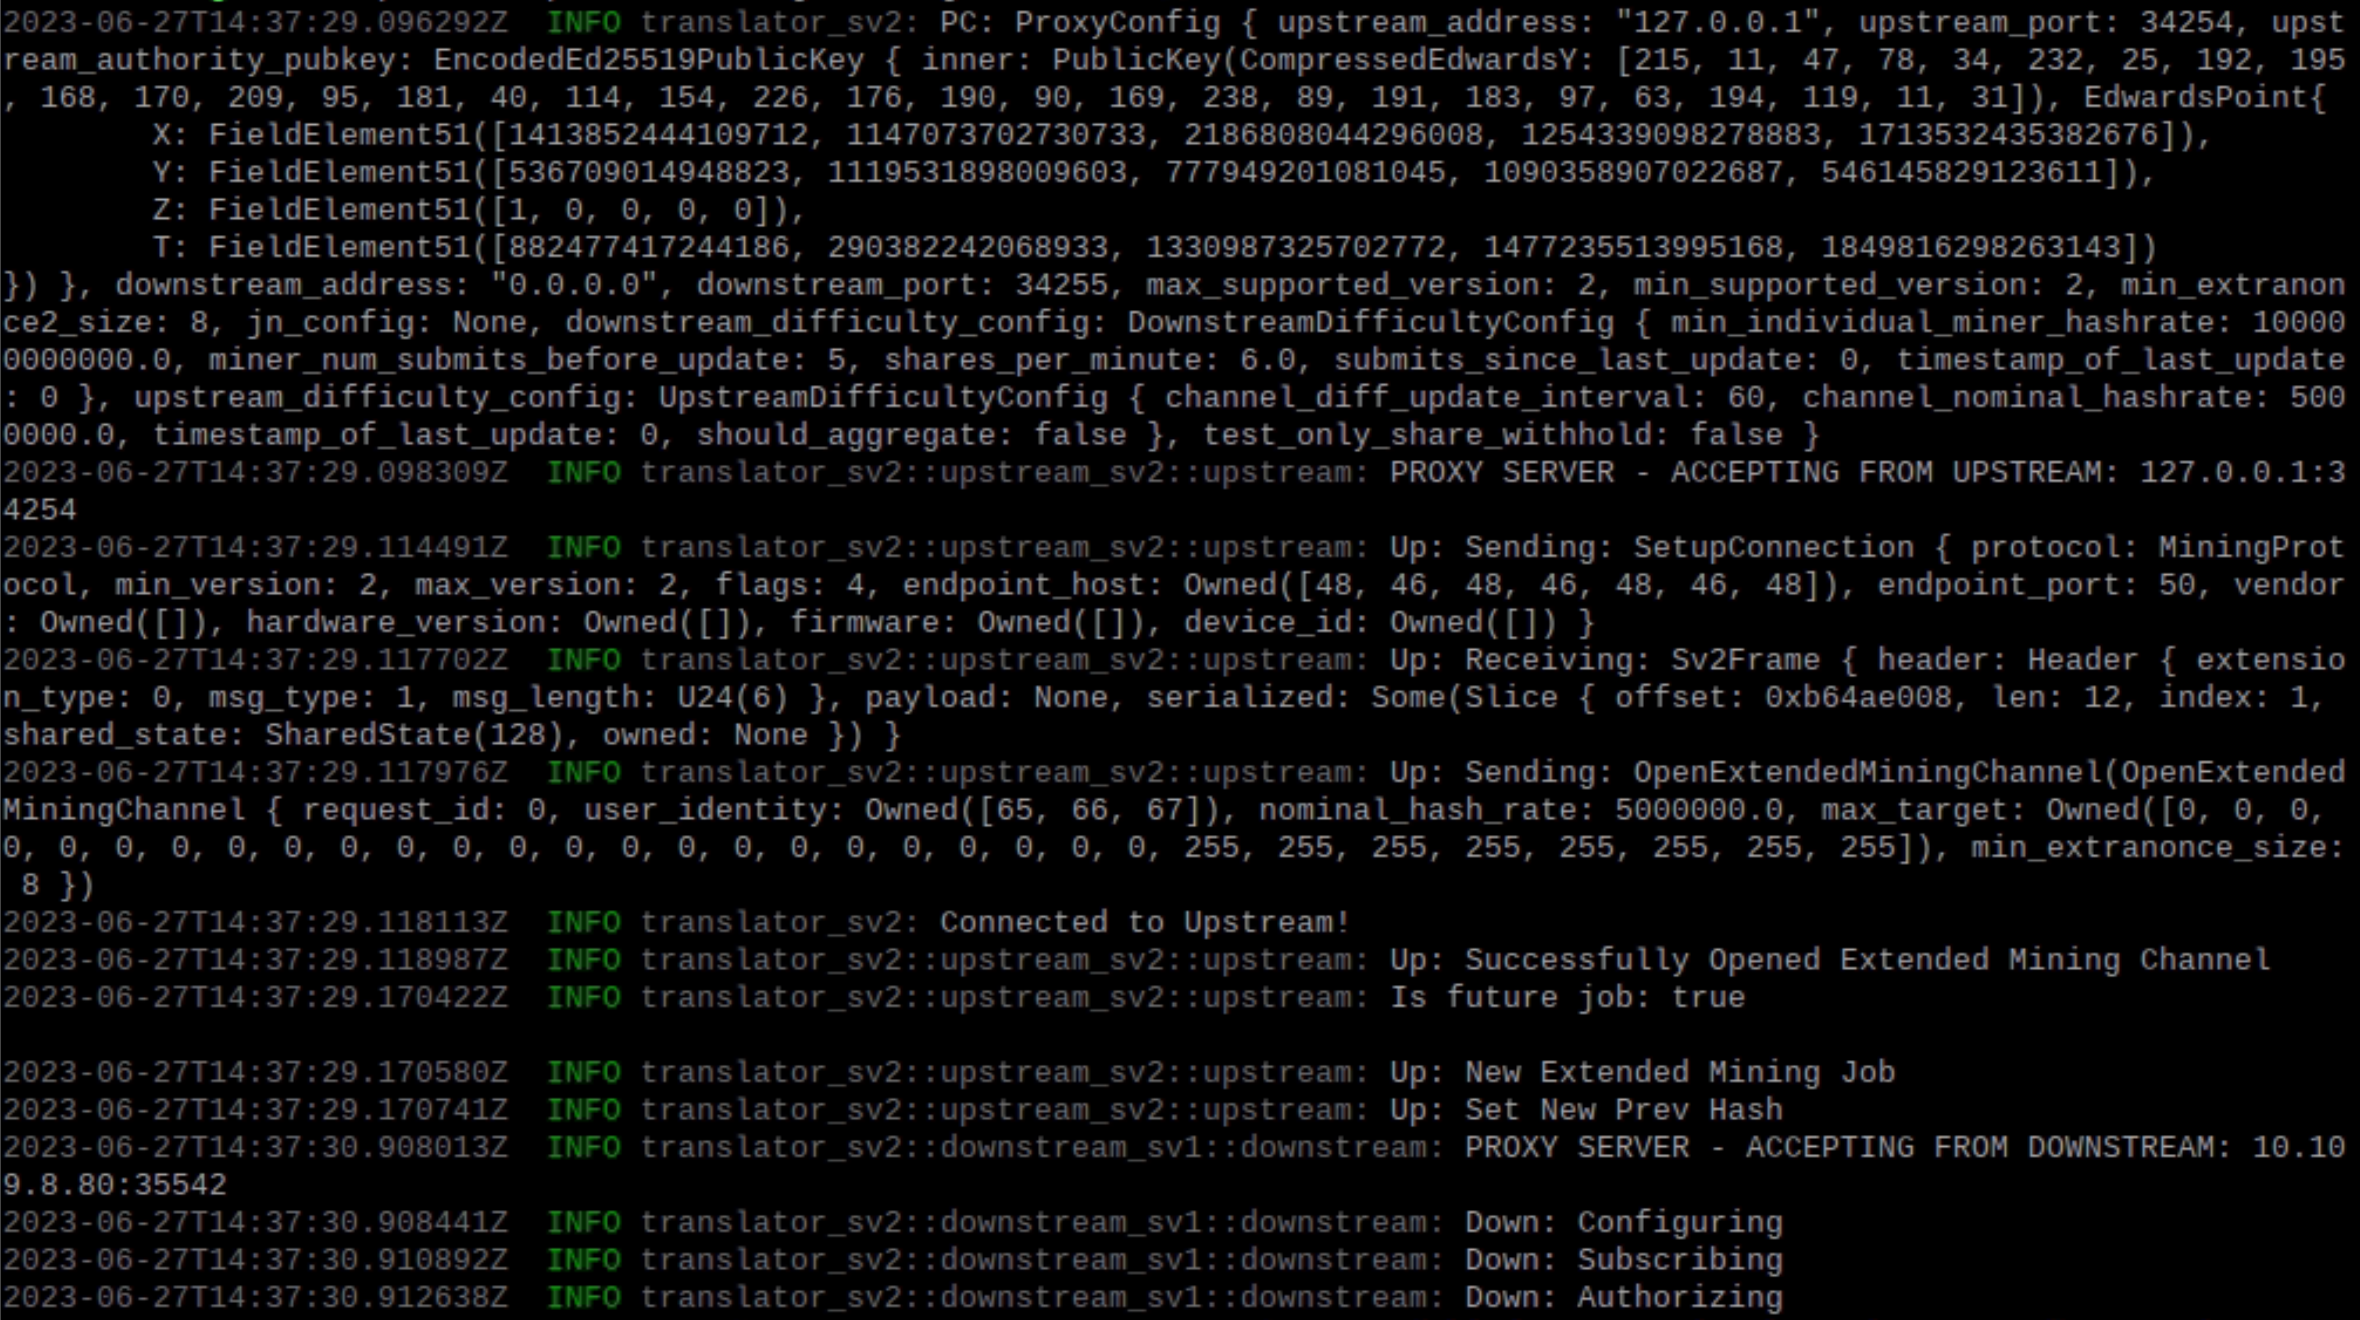
\includegraphics[width=15cm]{Figures/sri/sri_proxy.png}
    \caption{Translation Proxy logs successfully the ASIC miner SV1 requests}
    \label{fig:sri_asic_proxy}
    \end{figure}
    
\end{itemize}

\subsubsection{Config D}
As described in \ref{configD}, this configuration allows Mining Devices running SV1 firmware to connect to a SV2 Pool through a Translation Proxy (tProxy). In this case the tProxy is designed also to implement the Job Negotiation (JN) sub-protocol: allowing miners to select transactions locally and send them to the Pool-side JN. In the following guide a Template Provider (TP) is installed locally on the same machine, to provide block templates to the JN.\\
Since Config D is very similar to the configuration previously tested, the focus here wants to be on the \textbf{Template Provider} and \textbf{Job Negotiator} roles. \\

\noindent As already explained, here the big difference comes from the addition of the transactions selection feature: to let the miner locally do it, a \textbf{local Template Provider} is needed.\\
First of all, in a new terminal window:
\begin{lstlisting}[style=bashStyle, numbers=none]
    git clone https://github.com/stratum-mining/bitcoin.git 
    git checkout last-tested-tp 
    cd bitcoin/
    ./autogen.sh && ./configure --enable-template-provider
    make check
\end{lstlisting}
Once the local Template Provider (which is a version of Bitcoin Core full node with the ability to act as a SV2 TP) is installed:
\begin{lstlisting}[style=bashStyle, numbers=none]
    ./src/bitcoind -testnet
\end{lstlisting}
After checking that the TP is correctly running, the \textbf{SV2 Pool} server has to be run:
\begin{lstlisting}[style=bashStyle, numbers=none]
    cd stratum/roles/v2/pool/
    cp pool-config-example.toml ./conf/pool-config.toml
    cd conf/
\end{lstlisting}
Since the example config file is already configured to let the SV2 Pool connect to a local instance of Template Provider, nothing has to be changed in the configuration parameters. So, now run the SV2 Pool:
\begin{lstlisting}[style=bashStyle, numbers=none]
    cargo run -p pool_sv2 
\end{lstlisting}
As described in the command output, the Pool is now connected to the local Template Provider (127.0.0.1), and it will get the transactions to be put in the next block template from it.
\begin{figure}[h!]
    \centering
    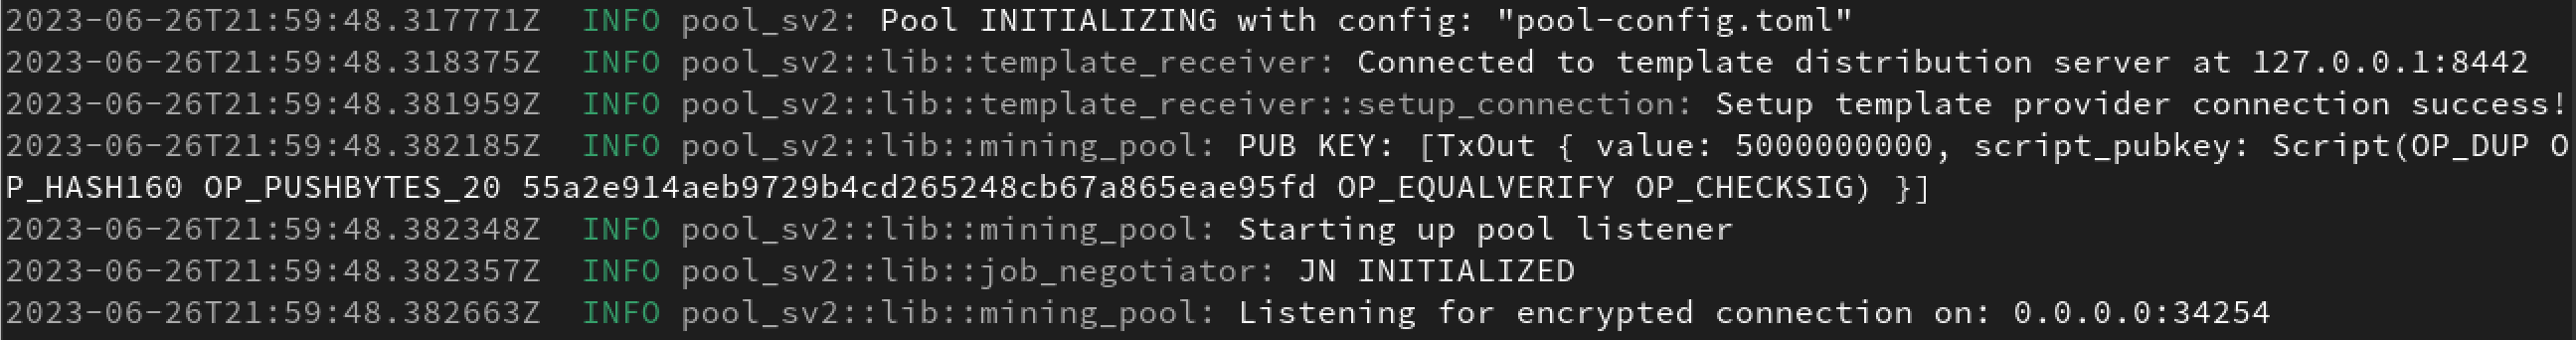
\includegraphics[width=15cm]{Figures/sri/configD_1.png}
    \caption{SV2 Pool connected to the local Template Provider, \textit{config D}}
    \label{fig:configD_1}
\end{figure}
\newline
\noindent At this point, like in the previous configuration tested, \textbf{the Translator Proxy} is needed. In a new terminal:
\begin{lstlisting}[style=bashStyle, numbers=none]
    cd stratum/roles/translator/
    cp proxy-config-example.toml ./conf/proxy-config.toml
    cd conf/
\end{lstlisting}
This time, since the Translator Proxy needs to act as a \textbf{Job Negotiator}, selecting the transaction from its own local Template Provider, some changes in its configuration file has to be done.
\begin{itemize}
    \item Uncomment the line 27 of the \textit{proxy-config.toml}, enabling the JNP. 
    \item Ensuring that line 31 (\textit{tp\_address = "127.0.0.1:8442"}) is uncommented. 
\end{itemize}
Now the Translator Proxy is ready to be run:
\begin{lstlisting}[style=bashStyle, numbers=none]
    cargo run -p translator_sv2 
\end{lstlisting}
\begin{figure}[h!]
    \centering
    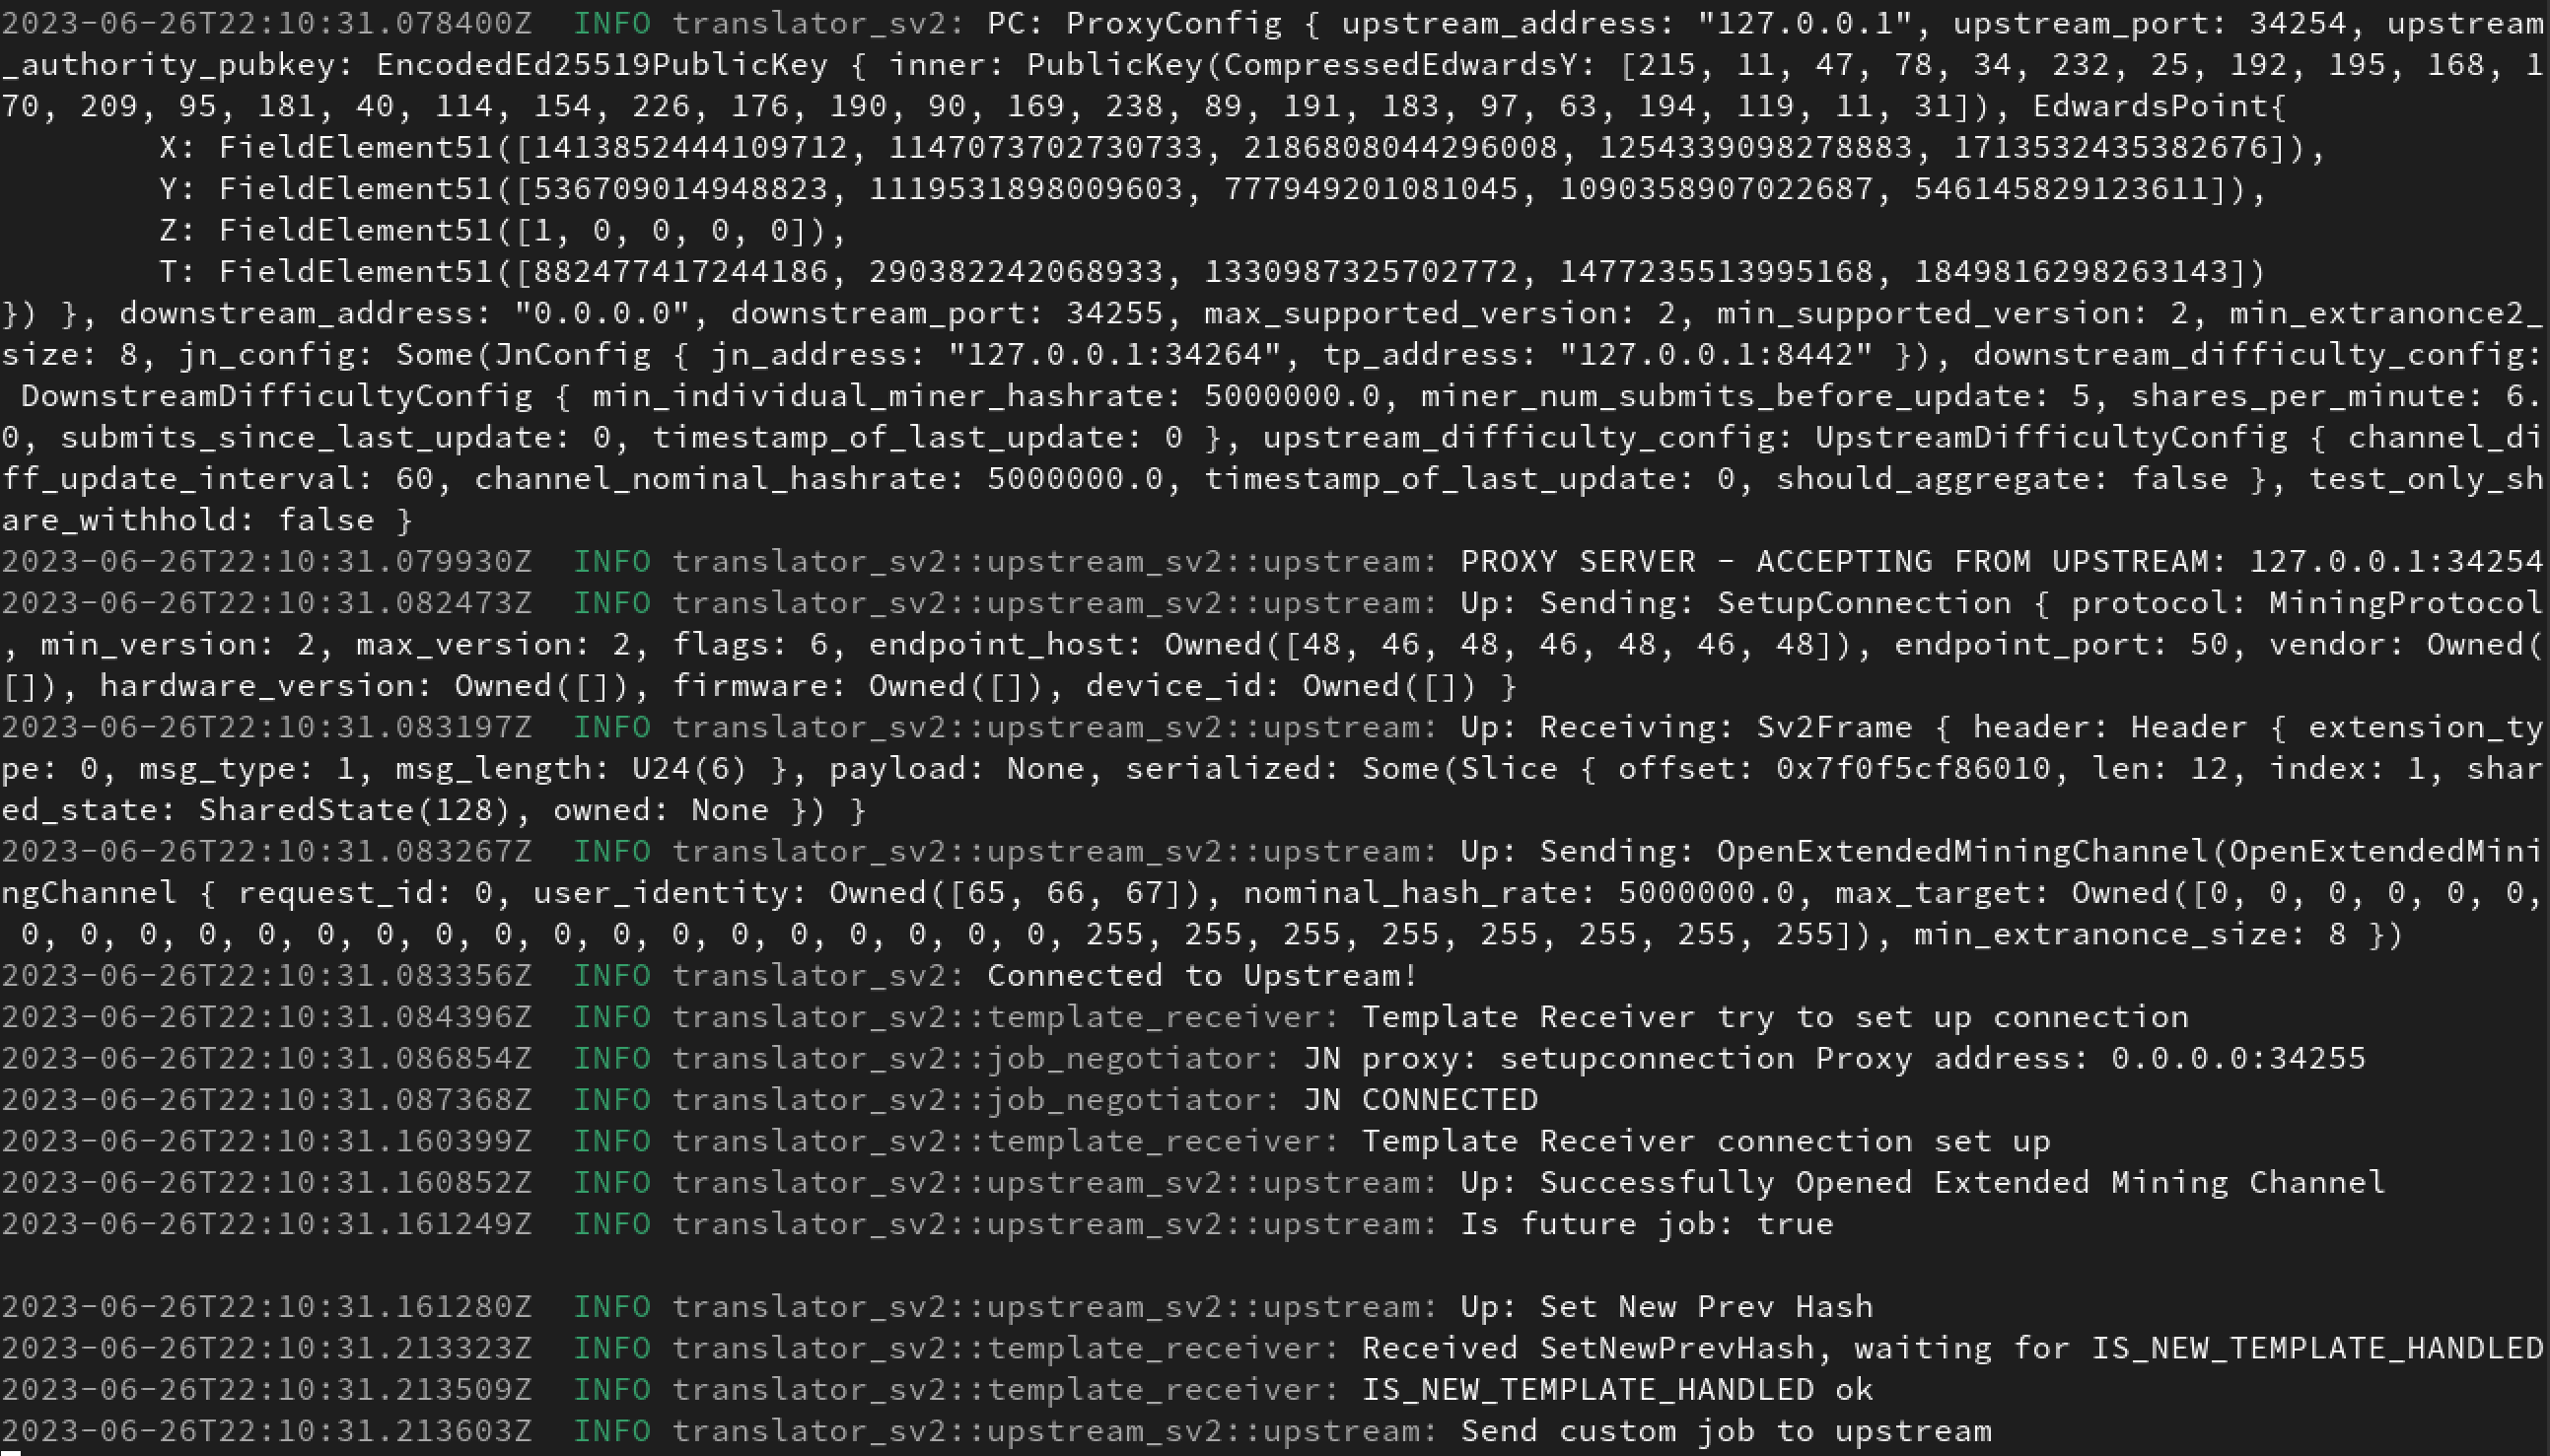
\includegraphics[width=14.5cm]{Figures/sri/configD_2.png}
    \caption{Translator Proxy which acts as a Job Negotiator, \textit{config D}}
    \label{fig:configD_3}
\end{figure}
As before, the Translator Proxy is now correctly running. This time, the big difference is inside the last log message of the command output:
\begin{lstlisting}[style=bashStyle, numbers=none]
    INFO translator_sv2::upstream_sv2::upstream: Send custom job to upstream
\end{lstlisting}

\noindent In this moment, as described in the logs of \ref{fig:configD_3} the Translator Proxy was able to create a custom job (block template to work on) using its own local Template Provider, and it communicated it to the Job Negotiator which is Pool-side!\\\\
However, since the details about the messages involved into the \textbf{Job Negotiator Protocol} are still material of discussions, the analysis about it won't go deeper than this. To be updated upon the final version and implementation details about this sub-protocol, it's suggested to have a look at \href{https://github.com/stratum-mining/sv2-spec/blob/main/06-Job-Negotiation-Protocol.md}{https://github.com/stratum-mining/sv2-spec/blob/main/06-Job-Negotiation-Protocol.md}.\\

\noindent Now, the only role which is missing is the \textbf{SV1 Mining Device}. And, as in the previous configuration, it will work with both CPU-miner and the real ASIC machine, in the same way described above.